\documentclass[11pt]{article}
\usepackage[top=1.00in, bottom=1.0in, left=1.1in, right=1.1in]{geometry}
\usepackage{Sweave}
\renewcommand{\baselinestretch}{1.1}
\usepackage{graphicx}
\usepackage{natbib}
\usepackage{amsmath}
\usepackage{gensymb}
\usepackage{parskip}
\usepackage{xcolor}
\usepackage[disable]{todonotes}
\usepackage{xr-hyper}
\usepackage[utf8]{inputenc}
\externaldocument{workingdraftsupp}

\def\labelitemi{--}
\parindent=0pt

\begin{document}

\renewcommand{\refname}{\CHead{}}

% See also: git/grants/crc2023/crc2023app/docs/crc_notes2023more.tex which has some reference notes

\title{Why longer seasons with climate change may \\ not increase tree growth} 
% Climate change highlights fundamental gaps in\\ plant growth $\times$ growing season length relationships  
% Do growing season length and growth relate? \\ And if not, why not? \\ And if we're not sure, why is that?
\author{Team Grephon}
\date{\today}
\maketitle



% We are a review or perspective, see https://www.nature.com/nclimate/content ... either way we need to be 3-5K words
\begin{abstract} % 195 words
A number of recent studies have challenged the fundamental assumption that longer growing seasons lead to increased tree growth, raising concerns that forecasts of future climate change---which include increased carbon storage through this assumption---may be overly optimistic. In a review of recent literature, we found that  58\% of studies supported the assumption of increased growth with longer seasons, while 36\% of studies did not. Diverging results remained when holding methodology constant. This suggests the current major challenge is to understand the biological mechanisms that underlie this widespread variation. Studies have proposed  a suite of hypotheses for why longer growing seasons may not always increase tree growth, including drought-related constraints and internal limits. These hypotheses and their underlying mechanisms, however, were generally tested in different ways by different fields, making comparisons difficult. We outline how bridging these current divides in hypotheses and methods while simultaneously integrating ecological theory could drive new advances in fundamental biology with major forecasting implications.  %...and help build a mechanistic framework for when longer seasons will---or will not---lead to greater growth, with implications of improve forecasts of forest responses and climate feedbacks in a warmer world.

% While studies have proposed  a suite of hypotheses for why longer growing seasons may not always increase tree growth, including drought-related constraints, internal limits, and methodological differences, comparing support for them is challenging given their diversity and that they were often confined to one sub-field: studies of tree ring growth tended to focus on external drivers, such as drought, while physiological studies of biomass or carbon allocation, tended to focus on internal limits, such as effects of photoperiod. 
\end{abstract}

\section*{Introduction} % about 4K plus 730 in boxes (4,550 words currently and by Jan 2024: Up to 5K ... feels a little too long to me, down to 4840 on 21 Feb 2024 ... down to 4K on 9 March ... but I assume that did not include boxes) on 27 May 2024: 4K plus 650 in boxes

The idea that longer growing seasons lead to increased plant growth is an intuitive tenet across multiple fields of biology, including physiology, dendrochronology and ecosystem ecology \citep{nobel1983biophysical,frank2022dendrochronology}. It is also a foundational assumption of many global carbon cycle models \citep[e.g.][]{friedlingstein2022global, ito2020global}. These models project that continued anthropogenic warming will be partly offset by increased carbon sequestration as warming lengthens growing seasons in many forests \citep{friedlingstein2022global}, an assumption supported by ecosystem-scale studies \citep{chen1999effects,keenan2014net,finzi2020}. 

Yet recent work has questioned this longstanding assumption \citep[e.g.][]{dow2022warm,green2022limits,silvestro2023longer}, with potentially large implications for future climate change. % This research suggests that limitations on plant growth mean forests could be limited sinks with increased warming, despite longer growing seasons. 
These recent studies challenge decades of research reporting increased growth with longer seasons, from observations along elevational and latitudinal gradients \citep[][]{myneni1997increased,berdanier2011growing,king2013tree,cuapio2022there}, classic experiments in lab settings \citep{went1957experimental}, to trends in ecosystem fluxes with warming \citep{chen1999effects,keenan2014net,finzi2020}. Proposed mechanisms for the apparent disconnect are diverse (Fig. \ref{fig:hypotheses}), including the complex nature of climate change \citep[e.g. drought or heat stress,][]{dow2022warm} and internal limits on plant growth  \citep{zohner2023effect}. % as well as inconsistent use of growth and growing season metrics and definitions \citep{green2022limits,korner2023four}.
% Studies that Green \& Keenan say no relationship:
	% Fatichi et al. 2014 (opinion)
	% Fatichi et al. 2019 (review)
	% JIang et al 2020 (FACE or sinilar) 

% Our approach spans multiple fields to unify foundational studies with recent research related to anthropogenic warming. Leveraging a systematic literature review, we examine in which methods, species and approaches extended seasons appear to lead to increased growth, and the current proposed hypotheses. 
Here we review methods and metrics used in diverse fields to uncover connections between growing season length and tree growth and identify the potential mechanisms that unite---and could disconnect---these processes. % Our approach spans multiple fields, from foundational to recent studies.  
Results suggest that predictable---and substantial---variation in growth $\times$ season length relationships across species exist. However, we also find a pervasive disciplinary split between studies, which often test different mechanisms on different species, and overlook insights from community and phylogenetic ecology \citep[e.g.][]{Grime:1977sw,Ackerly:2009ly,avila2023evidence}. We therefore argue that increased cross-disciplinary efforts would allow the field to rapidly develop a unified theoretical framework to predict when, where and how climate change may increase tree growth. % with implications both for forecasts of future climate change and fundamental science.
 % JHRL(Nov2023): I know this would make the sentence long, but I want to say that we are primed to get the insights but only if we take the opportunities (lizzie adds: And make the first sentence much more exciting; maybe move up: we highlight critical insights from physiology, community ecology, evolutionary and life history theory that have been unexamined in recent work)

\section*{Evidence that longer seasons increase plant growth, or not}
%  (spanning 36 papers and 59 unique tests or studies; see Supp or Fig/Table)
The idea that time limits growth is a fundamental principle across biology. Many biological processes---including photosynthesis and aspects of growth---are rate-limited, making time a crucial commodity \citep{nobel1983biophysical,cosgrove2005growth,hilty2021plant}. Thus, the hypothesis that longer growing seasons should increase growth is intuitive---and pervasive. 

Multiple fields have long assumed that longer seasons yield more growth. Foundational evidence comes from spatial clines across elevation and latitude, with growth decreasing alongside growing season length at higher elevations (Fig. \ref{fig:gxelev}) and latitudes. Experimentally, this assumption is supported by small-scale field warming studies that find that phenologically advancing species also grow more with warming \citep[][]{Cleland:2012}, while observationally, ecosystem-scale studies have reported a similar positive relationship between season length and carbon fluxes across decades with global warming \citep{keenan2014net} or in years with warm, early springs \citep{chen1999effects}. However, some recent studies do not support these previous findings.  These studies, which often focus on inter-annual correlations with metrics of standardized individual tree growth \citep{dow2022warm,silvestro2023longer}, have generated debate about whether future carbon storage forecasts are overestimated and which metrics of growth \citep{green2022limits}, or growing season length \citep{korner2023four}, are relevant.

Despite this recent debate, we found little support for a wholesale disconnect between growth and growing season length---instead finding split support for when longer seasons lead to increased growth. Papers spanning 25 years have variously found evidence for---or against---the relationship, with no clear pattern by method or year (Fig. \ref{fig:heatmaps} and see `Literature review methods' in Supplement). For example, carbon assimilation studies were evenly split in finding evidence for or against the relationship---or simply not testing it (Fig. \ref{fig:heatmaps}). Diverging results were consistently found within methods, suggesting the drivers of this variation are likely due to biological mechanisms, not solely inconsistent definitions of growth or growing season length \citep[as some, e.g. ][have recently suggested]{green2022limits,korner2023four}. 

Most studies explicitly tested the hypothesis that longer seasons with climate change increase growth via either increased time to grow (10 of 36 papers) or because longer seasons are usually warmer (8 papers), although many also considered hypotheses that could disconnect growth from season length. Studies from dendrochronology (the study of tree rings and their dating) and physiology have readily offered explanations for findings that increased growth may not be a universal outcome of longer seasons (Fig. \ref{fig:hypotheses}). External climatic drivers that offset the positive growth effects of longer seasons are often reported in tree ring studies \citep{kolavr2016response,de2022temperature,camarero2022decoupled}. In particular, the hypothesis that higher temperatures paired with lower precipitation produce negative correlations of season length with growth appeared in 58\% of tree ring studies we reviewed (and was only mentioned once outside of these studies, see also Fig. \ref{fig:hypotheses}). In contrast, 45\% of lab experimental and wood phenology (xylogenesis) studies suggested fundamental internal constraints that prevent trees from responding to longer seasons \citep[Fig. \ref{fig:heatmapssupp},][]{cuny2012life,michelot2012comparing,zohner2023effect}. Yet we found that these hypotheses have been tested in radically different ways, never together, and all ignore a suite of relevant research from other disciplines. % As we outline below, a single mechanism is unlikely to explain all results, requiring a more unified framework---and tests of it---for progress. 
 
\section*{Controllers on growth $\times$ season length relationships}

% A suite of mechanisms could prevent a universally positive growth $\times$ season length relationship. 
Studies have uncovered a suite of major mechanisms that could limit or disrupt the positive effects of longer growing seasons. These generally fall into two categories: (1) external factors, such as drought, which should impact ecosystem-level trends at regional scales, and (2) internal physiological constraints, which some research suggests are either universal across plants \citep[e.g.][]{zohner2023effect}, or species- and population-specific \citep[e.g.][]{soolanayakanahally2013timing}. The importance of these two factors, however, likely vary by species, highlighting the need to integrate perspectives from community and phylogenetic ecology. 

\subsection*{External drivers}

% \paragraph{Temperature \& moisture} % Abiotic
Fundamentally, temperature limits many biological processes. Temperatures that are too cool (below 5\degree C for temperate trees) and too warm \citep[an area of active research, but likely between 35-45\degree C;][]{martinez2008hot,cabon2022cross} slow down biological processes and eventually can lead to tissue death \citep[see Fig. \ref{fig:temperaturecomplex},][]{larcher1980,kramer2012book}. Between these upper and lower limits, biological processes underpinning growth generally accelerate such that warming can have a direct effect, by accelerating biological time, up until the maximum rate for that particular process. Assuming a common growth response curve to temperature, increased growth should be predictable at an ecosystem-level based on the current seasonal temperatures and the amount of warming. 

Positive effects of longer seasons on growth, however, could be counteracted by moisture deficits from reduced precipitation or higher evaporative demand (commonly invoked in tree ring studies (Fig. \ref{fig:hypotheses}). Support for this hypothesis comes from negative correlations between growth and precipitation or other metrics related to plant access to water in tree ring studies \citep{kolavr2016response,etzold2022number}. While we found drought limitation was far less considered in physiologically-focused studies, the mechanism is well supported by physiological observations that tree water status can be a biophysical limit to growth \citep[i.e., cells cannot expand without sufficient turgor,][]{peters2021turgor,cosgrove2023structure}, driving diel correlations between vapor pressure deficit and growth \citep{babst2019twentieth,zweifel2021trees}.
% Temperature response curves assume sufficient moisture, with growth rapidly slowly ....

Even without the complicating factor of soil moisture, the non-linear effect of temperature on photosynthesis can also limit growth responses (Fig. \ref{fig:temperaturecomplex}). At very cool temperatures---such as in early spring---a small increase in temperature may have limited effect, while an increase at warmer temperatures---such as those more common in the summer (e.g. 16 to 18\degree C)---could have a larger physiological impact. However, warming that pushes plants beyond their optima, where many biological rates crash, could have large negative impacts \citep{nobel1983biophysical,leuning2002temperature}. Thus, some studies hypothesize that longer seasons effectively only extend the very cool early-season periods and may have no discernible effect on growth, while other studies---based on tree rings---suggest that any increases in growth due to longer seasons are offset by reduced growth due to high summer temperatures \citep[Fig. \ref{fig:hypotheses},][]{gantois2022new,dow2022warm}. In contrast, other researchers argue that warmer temperatures to date have not have pushed trees above their optima \citep{schaber2002evaluation}, and instead have driven increases in growth through higher growth rates, rather than longer seasons \citep[e.g.][]{ren2019}. 

%\paragraph{Biotic interactions} 
Biotic interactions---including herbivory, disease and competition---can also act as external factors that limit growth, and may themselves be responsive to an extended growing season. For example, herbivory can have large impacts on forests, leading to declines in satellite measures of greenness often associated with plant senescence \citep{senf2017remote}}. Plant pathogens are also known to respond to warming, and are known to limit productivity \citep{sturrock2011climate,la2008forest}. These biotic drivers of growth were rarely mentioned in studies examining growing season length (we found no mention of them, Fig. \ref{fig:hypotheses}e), but could increasingly limit growth as extended growing seasons allow for additional generations of pests and pathogens \citep{mitton2012mountain,lange2006thresholds}.
% Kavya Nov2023: maybe we can connect this bit more to the hypothesis figure by mentioning the increased risk with an earlier growing season as an example of how herbivory/pests might impact growth

\subsection*{Internal constraints}
%  \paragraph{Universal limits \& triggers} 
When and how growth is initiated and ceases is under genetic and developmental control, and thus plants' internal programming could limit growth responses to longer seasons \citep{marchand2021timing,mckown2016impacts,soolanayakanahally2013timing}. Some recent studies suggest a novel role for the summer solstice \citep{zohner2023effect} in setting a universal developmental switch between when warming temperatures hasten or delay leaf senescence---thus influencing growing season length and growth. In contrast, decades of previous work imply such triggers are more complex, and vary at the population-level. 

Research has repeatedly shown that populations vary in their growth and its responses to extended seasons (Fig. \ref{fig:hypotheses}d), reflecting differences in genetic and developmental controls that likely evolved to limit tissue loss to rare early or late-season events. For example, populations often vary predictably in their end-of-season phenology, with more poleward populations tending to stop height growth (budset) earlier using locally adapted photoperiod cues \citep{soolanayakanahally2013timing,aitken2016}. This means longer seasons are generally driven by spring phenology, which appears far more flexible, and has advanced more rapidly than fall events \citep{aitken2016}. Within populations, individual trees may also vary in how early or late they initiate (spring) or end (fall) growth. This can be driven by a shifting investment to growth, survival and/or reproduction with growth. For example, saplings, for which growth and survival are paramount, tend to both grow more rapidly \citep{hilty2021plant} and have longer seasons relative to adult trees \citep{augspurger2003differences,rozendaal2010tropical,vitasse2014earlier}, which need to also invest in reproduction. % The response of adult trees may then vary depending on their investment in reproduction. 

Trade-offs between vegetative and reproductive investments may also produce important growth response differences across years within individuals, as well as between species. Years of high reproductive output can reduce growth \citep{thomas2011bookchptr,hacket2016tree}. For species that mast---producing abundant cones or fruits in only some years---high reproduction could especially impact measures of wood growth. Many hypotheses suggest higher summer temperatures trigger masting in the following year \citep{hacket2016tree,hacket2016consistent}; if true, then reduced growth in years following warm summers may not indicate temperatures too high for growth, as recent studies have suggested \citep[e.g.][]{gantois2022new,dow2022warm}, but instead shifting investment to reproduction.

\subsection*{Species-level variation}
% To date, a handful of studies have mentioned species differences (Fig. \ref{fig:hypotheses}) but almost none made or tested predictions on how species differ based on existing theory. 
The effects of these external and internal drivers on growth responses to growing season length are likely to vary across species, a reality rarely acknowledged by most studies \citep[Fig. \ref{fig:hypotheses}c. This despite the fact that species strongly predicts variation when studied, e.g.][]{cuny2012life,michelot2012comparing} with major implications for understanding the widespread observed variation in growth $\times$ season length relationships. Biogeographical patterns in climate and assembly within communities also predict species should evolve towards different optima and different strategies \citep{Ackerly:2009ly,buckley2012functional}. For example, leaf strategies (e.g. leaf mass per area, longevity) vary strongly between evergreen and deciduous species, but also within each group---where variation in `determinacy' defines the timing and investment of shoot growth and leaf emergence. Determinate species have most of their leaf material prebuilt in overwintering buds, generally unfolding their entire canopy within few weeks each season, while indeterminate species continue to produce new shoots including leaves over the growing season \citep{kikuzawa1982leaf,Lechowicz:1984cr}. Such differences would influence the extent to which the growth of different species respond to increases in growing season length, even under identical conditions. Current studies span a wide range of species (we found  57 species from 26 genera across 36 papers), making the aim of identifying a common relationship between growth and growing season length with current studies especially difficult.

% may27 (below paragraph: jhrl: This paragraph is more a suggestion for the future than the other paragraphs in these sections. Is that OK? ... jhrl: For example, we could delete this paragraph (making it more in keeping with other sections outlining the major reasons growth - growing season length relationships are not always positive), and then take a few of these ideas and move it to the next section (not sure were - maybe in models that push foward theory, especially if you leave out the 'towards forecasting' bit.). I'm not entirely sure that woudl work and also think it would be fine where it is, but thought I would include my thought processes in case useful. EMW: Cut and add 1-2 sentences to later where we mention this
Studies could leverage community and phylogenetic ecology theory to make useful predictions for when and where growth $\times$ growing season should be most apparent. Community ecology predicts trade-offs along an acquisitive to conservative axis, where some species grow rapidly and more flexibly to take advantage of resources, but are less defended against herbivores and compete poorly at low resource levels, whereas other species compete well at low resource levels, but at the expense of growing slower and conservatively \citep[][]{Grime:1977sw}. These ideas would predict indeterminate acquisitive species, such as poplar, to grow more with longer seasons, while conservative species, such as beech, may not. Functional traits could further refine these predictions, with where species fall along the acquisitive versus conservative trade-off defined by suite of leaf, wood and reproductive traits \citep[][]{diaz2016}. Under this framework, species with low leaf mass per area, diffuse vessels and consistent investment in fruit would show stronger shifts in growth with changing growing season length---assuming no other factors (e.g. drought or high temperatures) become limiting.

Phylogenetic ecology provides tools to study imprints of past selection which often shape species-level differences today, producing phylogenetic patterns that both limit how well species are adapted to current conditions and may constrain their responses to rapidly changing conditions \citep{Ackerly:2009ly}.  %Many species show evidence of previous selection, seen when evolutionary relationships (usually represented through phylogeny) predict plant responses and lead to clade-level similarities. 
Most studies testing for such historical effects on plant responses find them \citep[e.g.][]{phenophylo}, including new work on physiological traits \citep{avila2023evidence}, and previous physiological syntheses finding results suggestive of strong phylogenetic relationships \citep[e.g.][]{way2010differential}.

\section*{Building a new framework for growth $\times$ season length relationships} %
% Building a cross-disciplinary multi-level ...
% "Crossdisciplinary: viewing one discipline from the perspective of another. Multidisciplinary: people from different disciplines working together, each drawing on their disciplinary knowledge. Interdisciplinary: integrating knowledge and methods from different disciplines, using a real synthesis of approaches."
 % Building a mechanistic framework of when and where... 
Predicting when and where longer seasons lead to increased growth may seem overwhelming given the diversity of potential drivers and complexity of species-level differences we highlight. However, these broad sets of studies together offer a set of testable hypotheses that could rapidly advance progress---if tackled with a more cross-disciplinary approach. Such changes may take time, but major hypotheses can be tractably tested now. Taking advantage of existing data sets and ongoing experiments could provide tests of variation in growth---and potentially controllers on it---across individual to species and ecosystem scales, while new experiments can compare effects of external versus internal drivers on growth. Combining these in models that build up from internal limits to external drivers and include species-level variation would then provide predictions while helping to refine theory. More tractable changes within fields would also help - the high variation we found in observed growth responses to longer seasons across methods and even within species (Figs. \ref{fig:heatmaps}, \ref{fig:sppfinds}) could be partly reduced through standardized measurements (see Box: Standardized measurements) and a broadening of perspective within fields (see Box: Extending disciplinary focus). 
% This approach requires building fundamental biological knowledge in a suite of areas across physiology, dendrochronology, life history, ecology and evolutionary biology. These suggestions thus apply to understanding this relationship at the individual (organismal) level, though they make predictions at larger (e.g. ecosystem) scales, and are highly applicable to ecosystems dominated by one species \citep[e.g.][]{chen1999effects}. % These suggestions apply to those wanting to specifically address hypotheses about the relationship between growing season length, phenology and growth at the individual (organism) level

% A robust interdisciplinary approach to understanding growth $\times$ growing season length will need to integrate disciplines that focus on variation at the species-level and below. 


\subsection*{Using existing data and networks to partition levels of variation across drivers}

% may27 -- jhrl: I am a bit uncertain as to what this paragraph wants to do. Are we trying to say we need to better integrate across organizational levels? Or should we improve our understanding of what the relationship between growing season length and growth should be? Or is it both - we don't know what the relationship should be because we don't study these at the same levels of organization? ... jhrl: Generally, I find this paragraph (and the second part of the header "partition levels of variation" less clear than the existing opportunities (low hanging fruit) explained in the next paragraph. ... jhrl: OK - I now think I get it better when reading the next paragraph. Maybe switch the order and lightly edit? EMW: Or ... after discussion with JHRL: we thought move up the main message of ' While multiple papers report a lack of relationship between growth and growing season length, we have no fundamental understanding of what the effect size of this relationship should be, and thus no way to know if we have good power in current studies to detect it.' to intro of this final section (building framework) 
Predicting when longer seasons increase tree growth requires understanding the scale of growth variation at relevant organizing levels---individuals, populations, species, to provide a benchmark when comparing the effect sizes of external drivers of variation (e.g. climate, pest outbreaks). While multiple papers report a lack of relationship between growth and growing season length, we have no fundamental understanding of what the effect size of this relationship should be, and thus no way to know if we have good power in current studies to detect it. Estimates of how growth shifts with elevation (Fig. \ref{fig:gxelev}) likely include responses from both plasticity (within-individual variation) and local adaptation (population-level variation) and thus could be an upper bound on our expectations, yet elevational trends to date appear relatively weak and noisy---suggesting this is only part of our missing mechanistic understanding. However, a suite of current experiments, observational networks and existing databases could address this gap. 

Taking advantage of existing ecological and field global change experiments could help bridge across the two major fields currently studying growth $\times$ season length relationships---physiology and dendrochronology---and their contrasting timescales. We found most physiological studies of growth $\times$ growing season length relationships studied 1-2 years of dynamics, usually of juvenile trees, while tree ring studies focused on synthesizing across decades of adult tree growth. Perhaps because of this dichotomy, tree ring studies often study lag effects, while they are rarely mentioned in physiological studies, but current large-scale experiments on heat \citep[e.g. SPRUCE,][]{hanson2017attaining}, moisture via drought or irrigation \citep[e.g. DroughtNet, Pfynwald][]{smith2016drought} and other factors (e.g. $\text{CO}_2$ in FACE) have increasingly been used to test ecological `memory' \citep[e.g. ][]{flinker2021promise, schweiger2022transgenerational}. They thus could help scale up from smaller and shorter-time scales of physiological studies, potentially to ecosystem-level dynamics, such as carbon cycling \citep{ding2021plant,jensen2019simulated}. Building on available data and infrastructure could also bridge this gap, for example, adding dendrometers to provenance studies (and other common gardens) and locations with established phenological sampling and vice versa. Such efforts may be especially valuable in sites across elevational and latitudinal gradients (e.g. PSP, Feeley elevation network, Forest Inventory and Analysis). These sites in turn could be priority locations for xylogenesis and focused physiological studies. 

% Existing common garden studies on trees (often called `provenance trials' in forestry) provide an opportunity for more robust tests of population and individual variation. Given that many common garden studies have data on phenology \citep{aitken2016} and are designed to tease out population versus inter-annual variation, collecting tree ring data from them seems a rapid way to estimate variation across these two levels. New measurements of biomass or greenness within a growing season could also help compare support for whether internal limits are universal at solstice \citep{zohner2023effect}, variable by population \citep{soolanayakanahally2013timing}, or some mix.  % Given how old some common gardens are, research may also be able to examine impacts of biotic and abiotic disturbances or effects of climatic variation. 
% Common gardens not collecting regular phenology, or annual growth data, could start. 
% Common garden studies are designed to tease out population versus inter-annual variation, but the variation across these levels in growth $\times$ growing season length relationships is rarely studied. 

% may27 (below, first sentence): jhrl: Might this be a paragraph where to add some of the 'studies should consider' stuff mentioned in the previous section? Or if it is mostly suggested, maybe that paragraph can be deleted?
Existing open data repositories could test predictions from community ecology for species-level variation in responses to external drivers. Combining large-scale databases of tree rings and vegetative phenology (e.g. the International Tree Ring Database, ITRDB, and the Pan European Phenology project, PEP725, see Fig. \ref{fig:itrbdpep}) would provide a major spatially and temporally diverse dataset to compare how external climatic drivers, species and population together explain growth $\times$ season length relationships. While the low spatial and taxonomic overlap between these databases currently pose challenges (see Box: Extending disciplinary focus), these datasets may also allow us to identify  where longer growing seasons will increase growth and for which types of species. For example, combined databases could test the prediction that longer growing seasons will increase growth for species with regular reproduction \citep[no masting, see also new masting database in][]{hacket2022mastree+}, an acquisitive strategy, from clades that are historically (on an evolutionary timescale) plastic, in locations that are warm---but not too warm---and moist. 


\subsection*{New experiments to tease apart external \& internal drivers}

Given the complex effects of external drivers and internal constraints on growth $\times$ growing season length relationships, fully disentangling them will likely require new experiments. Changes in growing season length covary with other environmental changes, in particular longer seasons are usually warmer seasons \citep{ipcc2021}. Thus, experiments to robustly tease these drivers apart seem a paramount need, especially if done across multiple species spanning diverse strategies. Similarly, factorial experiments that manipulate season length (via early growth or delayed senescence), while additionally manipulating external abiotic (e.g. heat waves, droughts) and/or biotic (e.g. pests, competition) drivers could allow us to compare the effects of these drivers on tree growth. Such experiments could also test lag effects, if sampled multiple years after the manipulations (versus the common practice of destructive sampling at the end of the treatment growing season). While such experiments are most easily done for juvenile trees, they could also be done on adult trees, given investment in infrastructure. % Similarly, experiments to compare impacts of external biotic and abiotic drivers are critical---if carefully designed they would also provide insights on potential constraints.  

Efforts to design and launch such large-scale experiments should start now. Long-term experiments on adult trees that manipulate temperature, precipitation and growing season length could test a suite of drivers at relevant lifestages. Such experiments could robustly compare drivers and become a resource for testing the underlying mechanisms for constraints, if properly measured and designed. This would mean careful measurements of carbon allocation, including to reproductive output, and tissue lost to frost and biotic drivers, and choosing species to maximize divergent strategies and provide the potential for genomic and related studies (e.g. \emph{Populus, Quercus}). Given the potential role of evolutionary history, selecting for these varying strategies within a clade, or---if not feasible---correcting for phylogenetic distance would provide more robust tests of how strategies influence the growth $\times$ season length relationship. % Given an increasing number of studies across more species, a careful synthesis of studies across species could further test for the role of evolutionary history. 
These highly measured experiments  would represent a major investment to tackle this question in one location, and could form part of a broader network of sites that test these relationships at larger spatial scales. Distributed experiments to measure growth and phenology (ideally wood and vegetative) of multiple provenances of multiple species across sites could estimate variation---and potential constraints---that operate at different organizing levels. 

\subsection*{Models that push forward theory}
Efforts to bridge observational trends with experimental insights will need a variety of models, % may27 -- previous 'models' jhrl: do we just mean statistical models or also theoretical models? I would argue all? EMW: And better conceptual models ... rebuild section some (or move broader points up to opening of section?) 
both process-based and statistical (and ideally both), that can bridge across temporal and organismal scales while testing the major hypotheses. %Such models would ideally capture the potential inter-connections between external drivers, internal constraints and species-level differences in growth responses to warmer, longer seasons. 
% ... will require a new modeling framework to make useful predictions of growth responses to warmer, longer seasons across species, species and levels of warming. 
% may27 -- below -- jhrl: Right now this paragraph because of how it's worded primarily suggests we need to build better statistical mdoels, when I htink we also need better models of growth, no? I've tried to edit with this in mind
Such models should include the separate effects of temperature, moisture and growing season length while partitioning individual, population and species-level variation---thereby providing broad-scale estimates of the effects of the major external drivers versus potential internal constraints (which may be apparent as within-season and/or population differences). Including species-level effects while also integrating phylogenetic relationships between species could then test for the role of evolutionary history in shaping responses, while adding in site $\times$ year-level effects of biotic disturbances could begin to compare across abiotic and biotic external drivers. Such models should be built alongside a suite of mechanistic process-focused models that scale up. For example, one model could build from carbohydrate balance and cell division \citep[e.g.][]{locosselli2017dendrobiochemistry} to predict growth dynamics observed in xylogenesis, while another could build from phenology, including frost disturbance and reproduction, to predict growth \citep[e.g.][]{chuineJTB}. 

The success of modeling approaches will likely depend on how nimbly they respond to new findings, and how well they make predictions for new studies to test. As new experiments identify potential internal growth constraints and what level they operate on (universal, population or otherwise), both statistical and physiological process models should be adapted and improved. Together the interplay of statistical and more mechanistic process-focused models would likely provide major insights into the fundamental biology of how tree growth shifts with extended seasons, and yield a unified model for robust predictions of growth responses to warmer, longer seasons across species and levels of warming. 

\emph{Conclusions:} % FIX ME or cut, see some good text commented out below. 
Anthropogenic climate change has often been described as an unfortunate and unplanned experiment. Like many experiments, it has highlighted important biology we don't know well, requiring us to rediscover dusty old fundamentals, while also exposing the limits to our understanding. Understanding when, how and why longer seasons lead to increased tree growth requires an interdisciplinary reckoning with how temperature, time and a suite of external and internal drivers affect plant growth. The task may seem large, but bridging across theory and data from dendrochronology, physiology, community and phylogenetic ecology could rapidly advance fundamental biology in ways that translate directly to improved models of future forest dynamics, and the suite of species and services that depend on them. % And that includes carbon sequestration---which, we really need now! 

% Most fields studying growth $\times$ growing season length relationships consider a limited set of metrics and a small subset of possible drivers (see Figs. \ref{fig:heatmaps}, \ref{fig:heatmapssupp}). Beyond failing to test a suite of highly relevant mechanisms, the lack of interdisciplinary study means we lack coherent tests that compare multiple mechanisms. Taken together, the current landscape of research suggests we may be testing hypotheses for how plants shift with climate change that we never previously understood well in fundamental biology.
% Most fields studying this include a limited set of metrics and consider only a small subset of potential factors, with entire suites of hypotheses missing from the literature (see Fig. XX). 

% Beyond failing to test a suite of highly relevant mechanisms, the lack of interdisciplinary study means we lack coherent tests that compare multiple mechanisms. Dendrochronology considers almost exclusively external climatic drivers, while physiological tests of constraints do not usually predict for which species, when and where constraints will be most important. Taken together, the current landscape of research suggests we may be testing a hypothesis for shifts with climate change that we never previously understood well in fundamental biology. 

\emph{Acknowledgements:} B. Wuu for extracting growth $\times$ elevation data; R. Z{\"a}ch for logistical support; N. Pederson for discussion and J. Davies for comments that improved the manuscript. 

\iffalse

i. Hypotheses for why GSL x growth is not found are not equally tested across fields: Constraint issues in provenance but not tree ring etc.\\
ii. Our premise is that some hypotheses for what is going may be tractably already answered by combining data across fields/methods\\
iii. And, you could go far by cross-field tweaking of what each field is doing

Most global models of future warming assume increased anthropogenic carbon will be offset by increased carbon sequestration in forests as growing seasons lengthen.

The proposed mechanisms for this, however, are highly diverse---and most studies measure different aspects of growth across widely varying spatial and temporal scales. 

A positive link between longer growing seasons and increased carbon sequestration 

A suite of recent studies have called into question this fundamental assumption .... failed to find a link between longer seasons and increased tree growth

This assumption appeared well supported by several large-scale studies of ecosystem fluxes 
\fi


\newpage
\section{Boxes!}
\subsection*{Box. Standardized measurements} % ``Growth", measured how, exactly? ...

Understanding the diverse drivers and testing underlying hypotheses (Fig. \ref{fig:hypotheses}) for growth $\times$ growing season length relationships requires a common language. We found 14 different metrics of start, 16 metrics of end of season (25 metrics of growing season length), and 21 different metrics of growth across 59 studies---highlighting just part of the problem (see also \emph{The challenge of metrics: Measuring growth} in the Supplement). Definitions and metrics for external and internal drivers were myriad, %CJC 15Dec - I think we could again add numbers for external and internal divers, clarifying these were after systematically assigning studies into groups
with papers reporting dozens of tests of different aspects of climate over different temporal windows. Although this is understandable given the differing goals of these papers, this also slows progress. 

A common framework for explanatory and response variables would accelerate research by easing communication between fields and providing a path to comparable quantitative estimates. This should also include expected statistical tests, as we found a number of papers failed to directly test for growth $\times$ growing season length relationships (Fig. \ref{fig:heatmaps}), often instead testing only certain hypothesized indirect relationships \citep[e.g. spring temperature $\times$ growth in][]{dow2022warm}. % A first fundamental need for any framework is comparable quantitative estimates---which we currently lack. 

\subsection*{Box: Extending disciplinary focus to help bridge the internal-external drivers divide} 

% Careful interdisciplinary is critical, but will benefit from shifts within disciplines. 
% Standardized measurements will not yield fully comparable estimates---especially on the relative impacts of external and internal drivers---without larger shifts within fields. We found that dendrochronology considers almost exclusively external climatic drivers, while physiological tests of internal constraints do not usually make predictions that scale up easily beyond the lab or greenhouse. Major fields studying this relationship---dendrochronology, phenology research and physiology---all need to broaden in specific ways to overlap with one another to facilitate interdisciplinary work. At the same time, all fields have missed certain major hypotheses they could test (Fig. \ref{fig:hypotheses}), highlighting the need to integrate perspectives from other disciplines with relevant theory and methods. 

Each field studying growth $\times$ growing season length today has its own historical aims, and thus, its own biases towards certain species, methods and metrics. For example, dendrochronology's original focus on using tree growth to estimate climate has led to sampling biases \citep[e.g. to `climate-sensitive' individual trees,][]{klesse2018sampling,nehrbass2014influence} and statistical detrending \citep{rollinson2021climate}, which may obscure patterns where the signal of longer growing seasons and biotic drivers may be most apparent \citep[such as rapid growth phases,][]. Another example - dendrochronology generally focuses on conifers \citep[gymnosperms,][]{zhao2019international}, creating a major split from most studies of leaf phenology, which focus almost entirely on deciduous angiosperm species (see Fig. \ref{fig:itrbdpep}). By contrast, phenology research has been strongly focused on spring events (e.g. budburst, leafout), with limited data on fall events and thus limited data to calculate growing season length. This focus on spring events may have been justified decades ago, when most shifts from anthropogenic warming occurred in the spring, but less justified as increasing research suggests important complexity in fall shifts \citep{gill2015,zohner2023effect} and a need to scale up phenological research to understand tree growth.

%[jhrl deleted this - was too long] led to certain assumptions and methods that may obscure the complexity of how growth shifts with growing season length. Fundamentally, the field relies on an assumed relationship that, within individual and populations of trees, growth (measured by annual ring width) is greater when growing conditions---climatically---are better \citep[e.g.][]{cook2013methods}.  Dendrochronologists' traditional aim to magnify this climate signal has led to standard approaches, including sampling biases \citep[e.g. to `climate-sensitive' individual trees,][]{klesse2018sampling,nehrbass2014influence} and statistical detrending \citep{rollinson2021climate}, that may obscure patterns where the signal of longer growing seasons and biotic drivers may be most apparent \citep[such as rapid growth phases,][]{manzanedo2019towards}.  %Fundamentally, the field has long assumed growth decreases with shorter growing seasons \citep[e.g.][]{bruening2017} over space, such as higher elevations and latitudes.%AKE: I have not read bruening but a skim of it suggests that it is not a tree ring paper- rather a treeline paper. do we still want to cite it here? I removed it but I can look for another one that is tree ring focused...
 % Bridging this gap would be aided by physiological studies reporting metrics similar to ring width, alongside their more common measurements of shoot elongation, height and biomass. 

These field-specific historical trends limit the opportunities for interdisciplinary insights. For example, dendrochronology studies generally eliminate much of the drivers that physiological studies focus on. Opportunities to overlap dendrochronology time records with metrics of growing season length measured through vegetative phenology appear high, but sampling biases towards conifers in one and angiosperms in the other field limit current opportunities. All fields could therefore benefit from tackling the challenge of understanding the physiological connections between growing season length and growth, and even the genetic and developmental underpinnings of these connections. To date, much work has focused on measures of growth and phenology without a clear mechanistic understanding of what triggers growth and its cessation, and how these triggers and responses have evolved.  %CJC 15 Dec - reference Fig S1 here - only 3 studies looked at external or internal factors by phenology.
Progress in this area could be particularly important for making projections, as extrapolating can be dangerous when the underlying mechanistic model is wrong. Physiological studies that follow carbohydrate balance and cell division \citep[see][]{locosselli2017dendrobiochemistry} versus growth dynamics could yield insights, as could additional work on xylogenesis---especially if done with a focus both to extrapolate to long-term tree ring studies and/or in physiological experiments \citep{fang2020physiological,simard2013intra}. Expanding beyond the current disciplines focused on this topic could also be informative. For example, a clearer physiological understanding of which environmental stimuli trigger leaf expansion, senescence, woody growth, and heartwood formation alongside an evolutionary perspective could advance understanding of growth
constraints \citep{baas2011wood,eckert2019makes,ensminger2015tree,juvany2013photo}.

% Biotic/spp diversity for all ... 
% All fields have lacked a focus on the ecology of growth $\times$ growing season length, generally ignoring impacts of certain external drivers, the complexity of life-history, and species differences. Dendrochronology often uses frost events or insect outbreaks as markers of particular years, but rarely integrates them into patterns of growth. A shift to reporting and estimating effects of frost events, biotic disturbances, and reproduction status of trees (including mast years) could provide new estimates of the effects of these drivers. Physiological studies tend to avoid such complexities through controlled environments and a focus on juvenile plant stages  \citep{poorter2016pampered}, but scaling up between life stages will be critical for useful models of growth, and to bridge to dendrochronology. % Both fields have also tended to ignore competition. Mechanistic physiology studies rarely measure or include competition and, given dendrochronology's focus on climatic signal through growth, the field similarly tries to avoid the study or impact of plant competition, even though it is foundational to forest dynamics.

% All fields would benefit from a deeper understanding of the physiological and/or developmental connections between growing season length and growth. Much work has focused on measures of growth and phenology without a clear mechanistic link. Similarly, many current suggestions of constraints lack any physiological mechanism. Physiological studies that follow carbohydrate and cell division versus expansion dynamics could yield insights. This is particularly important if want to include constraints in our projections, as extrapolating is especially dangerous when the underlying mechanistic model is wrong

\newpage
\section{Figures}


\clearpage
\begin{figure}[h!]
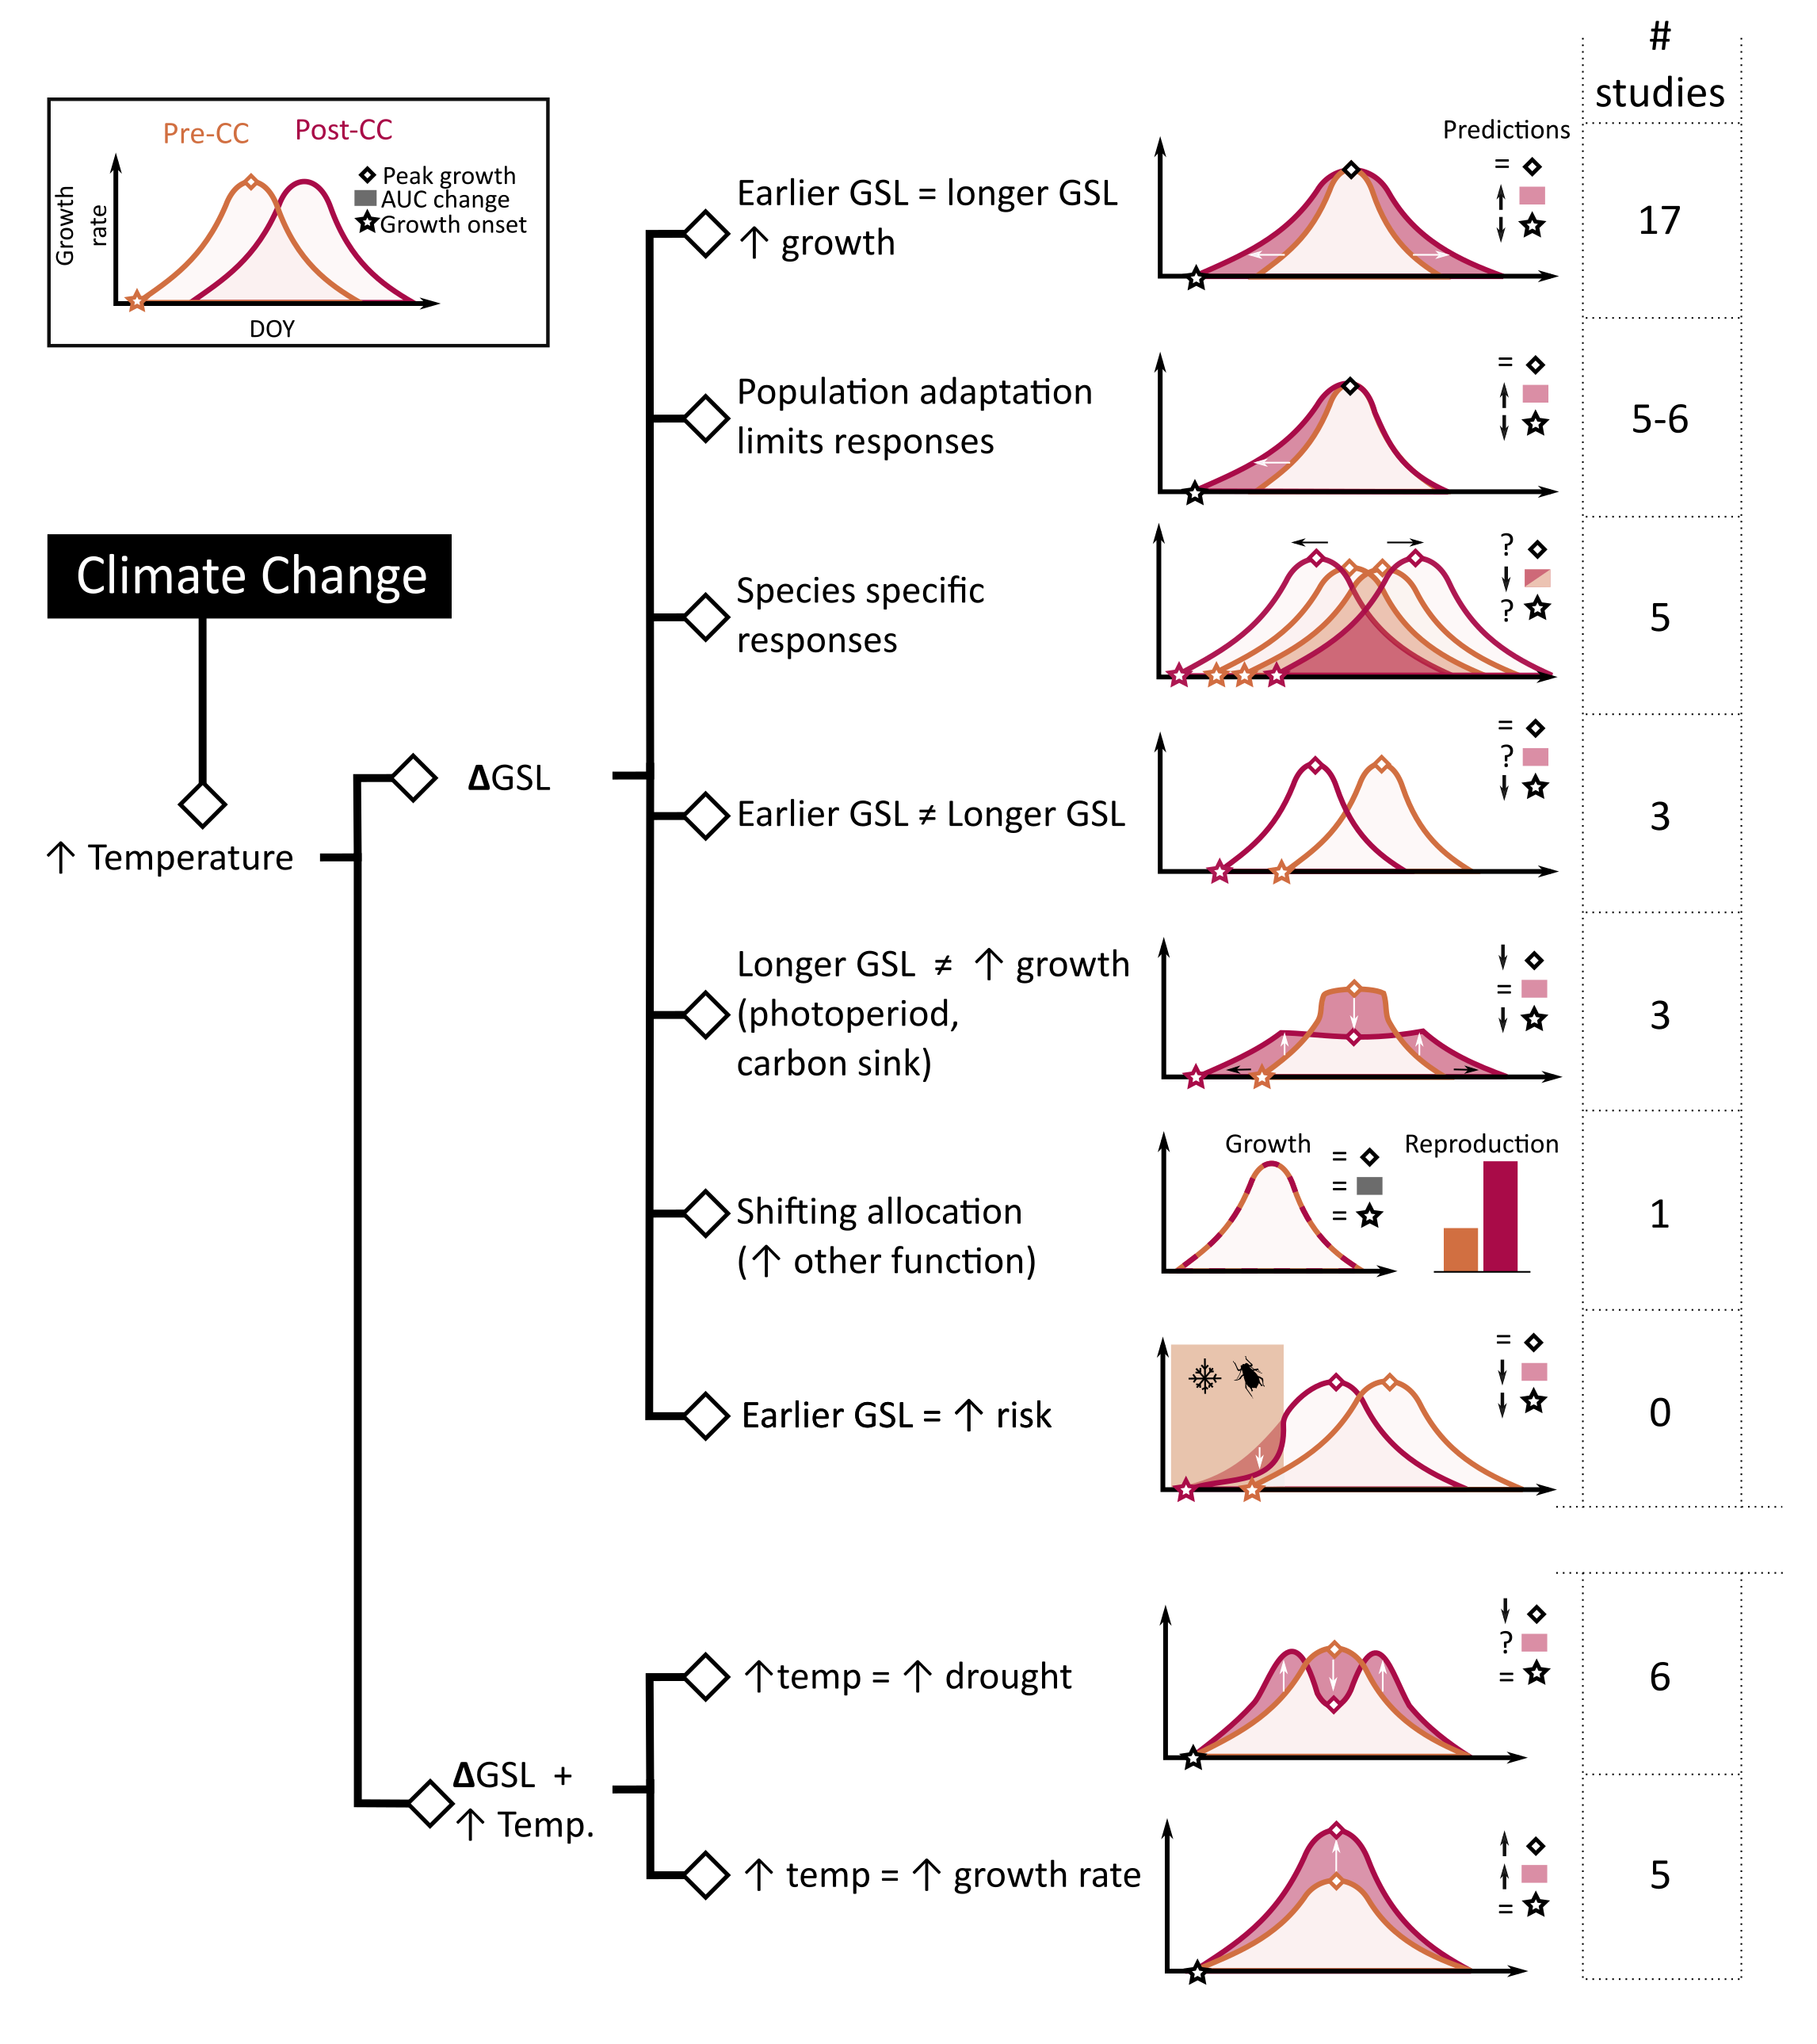
\includegraphics[width=0.9\textwidth]{..//figures/hypothesesconceptfig.png}
\caption{Pathways through which climate change could alter growing season length and growth.} % TRY to add source/sink maybe? % Hypotheses focus on both source (photosynthesis-limited, including $CO_2$ limitation) and sink limitations ....

\label{fig:hypotheses}
\end{figure}

\begin{figure}[h!]
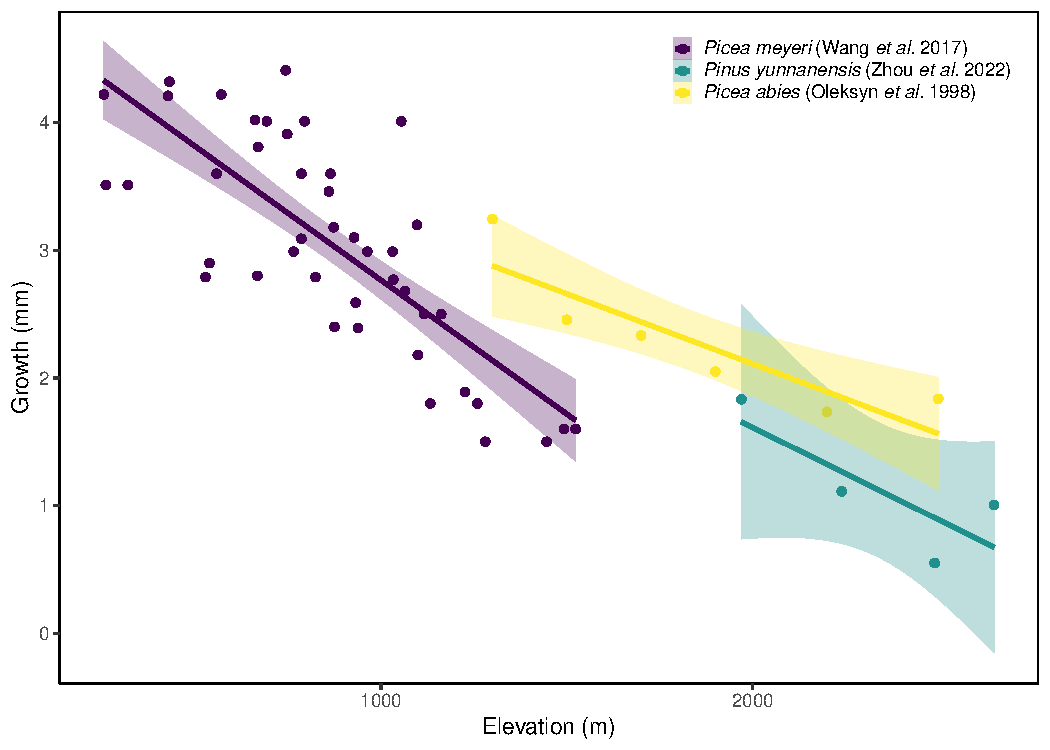
\includegraphics[width=0.8\textwidth]{..//analyses/growthxelevationetc/figures/growthbyelevation_plot.pdf}
\caption{Growth $\times$ elevation relationships from the literature with simple linear regression fits shown with 89\% confidence intervals. Oskelyn measured growth (mm) as diameter at breast height increments, while the other studied measured it ring width. See Supplement for more methods details and Fig. \ref{fig:growelevMORA} for an example from one site.}
\label{fig:gxelev}
\end{figure}

\clearpage
\begin{figure}[h!]
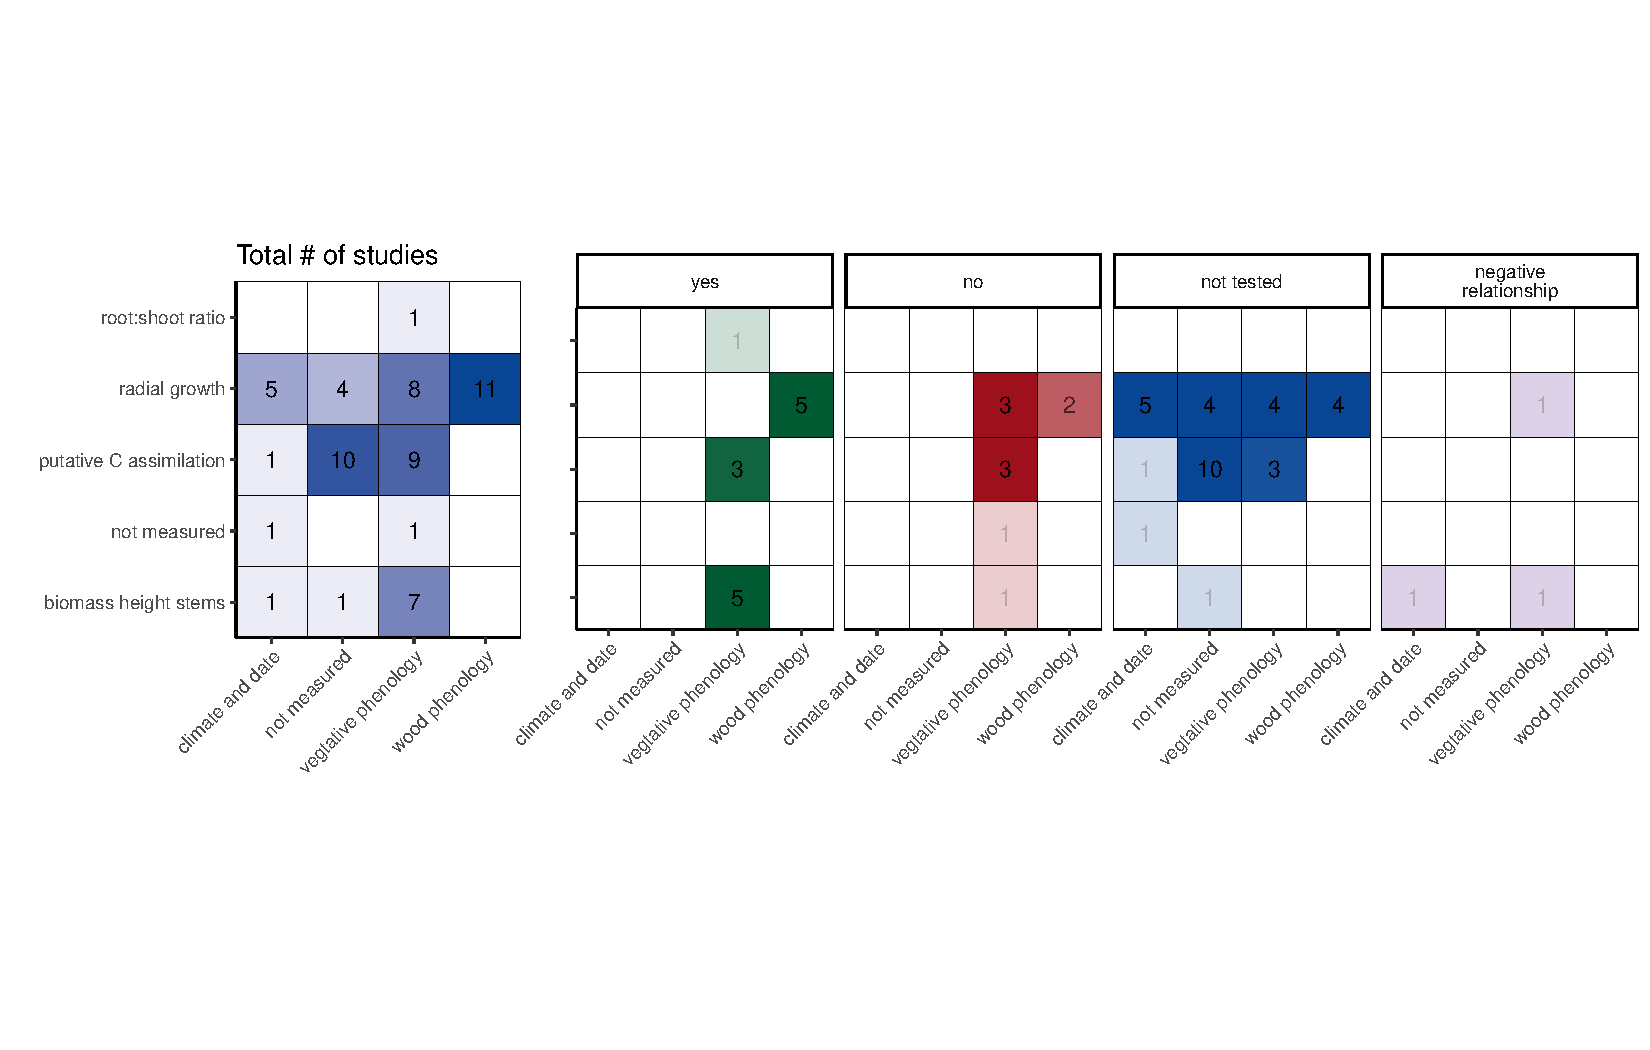
\includegraphics[width=1\textwidth]{..//figures/heatmaps/combinedheatmap_gslxgrowth_simple.pdf}
\caption{A review of growth $\times$ growing season length relationship studies spanned a diversity of methods, but there was no coherency in which methods did or did not find a positive relationship. Not directly testing for the relationship was surprisingly common across methods. See Supplement for review details.}
\label{fig:heatmaps}
\end{figure}

\clearpage
\begin{figure}[h!]
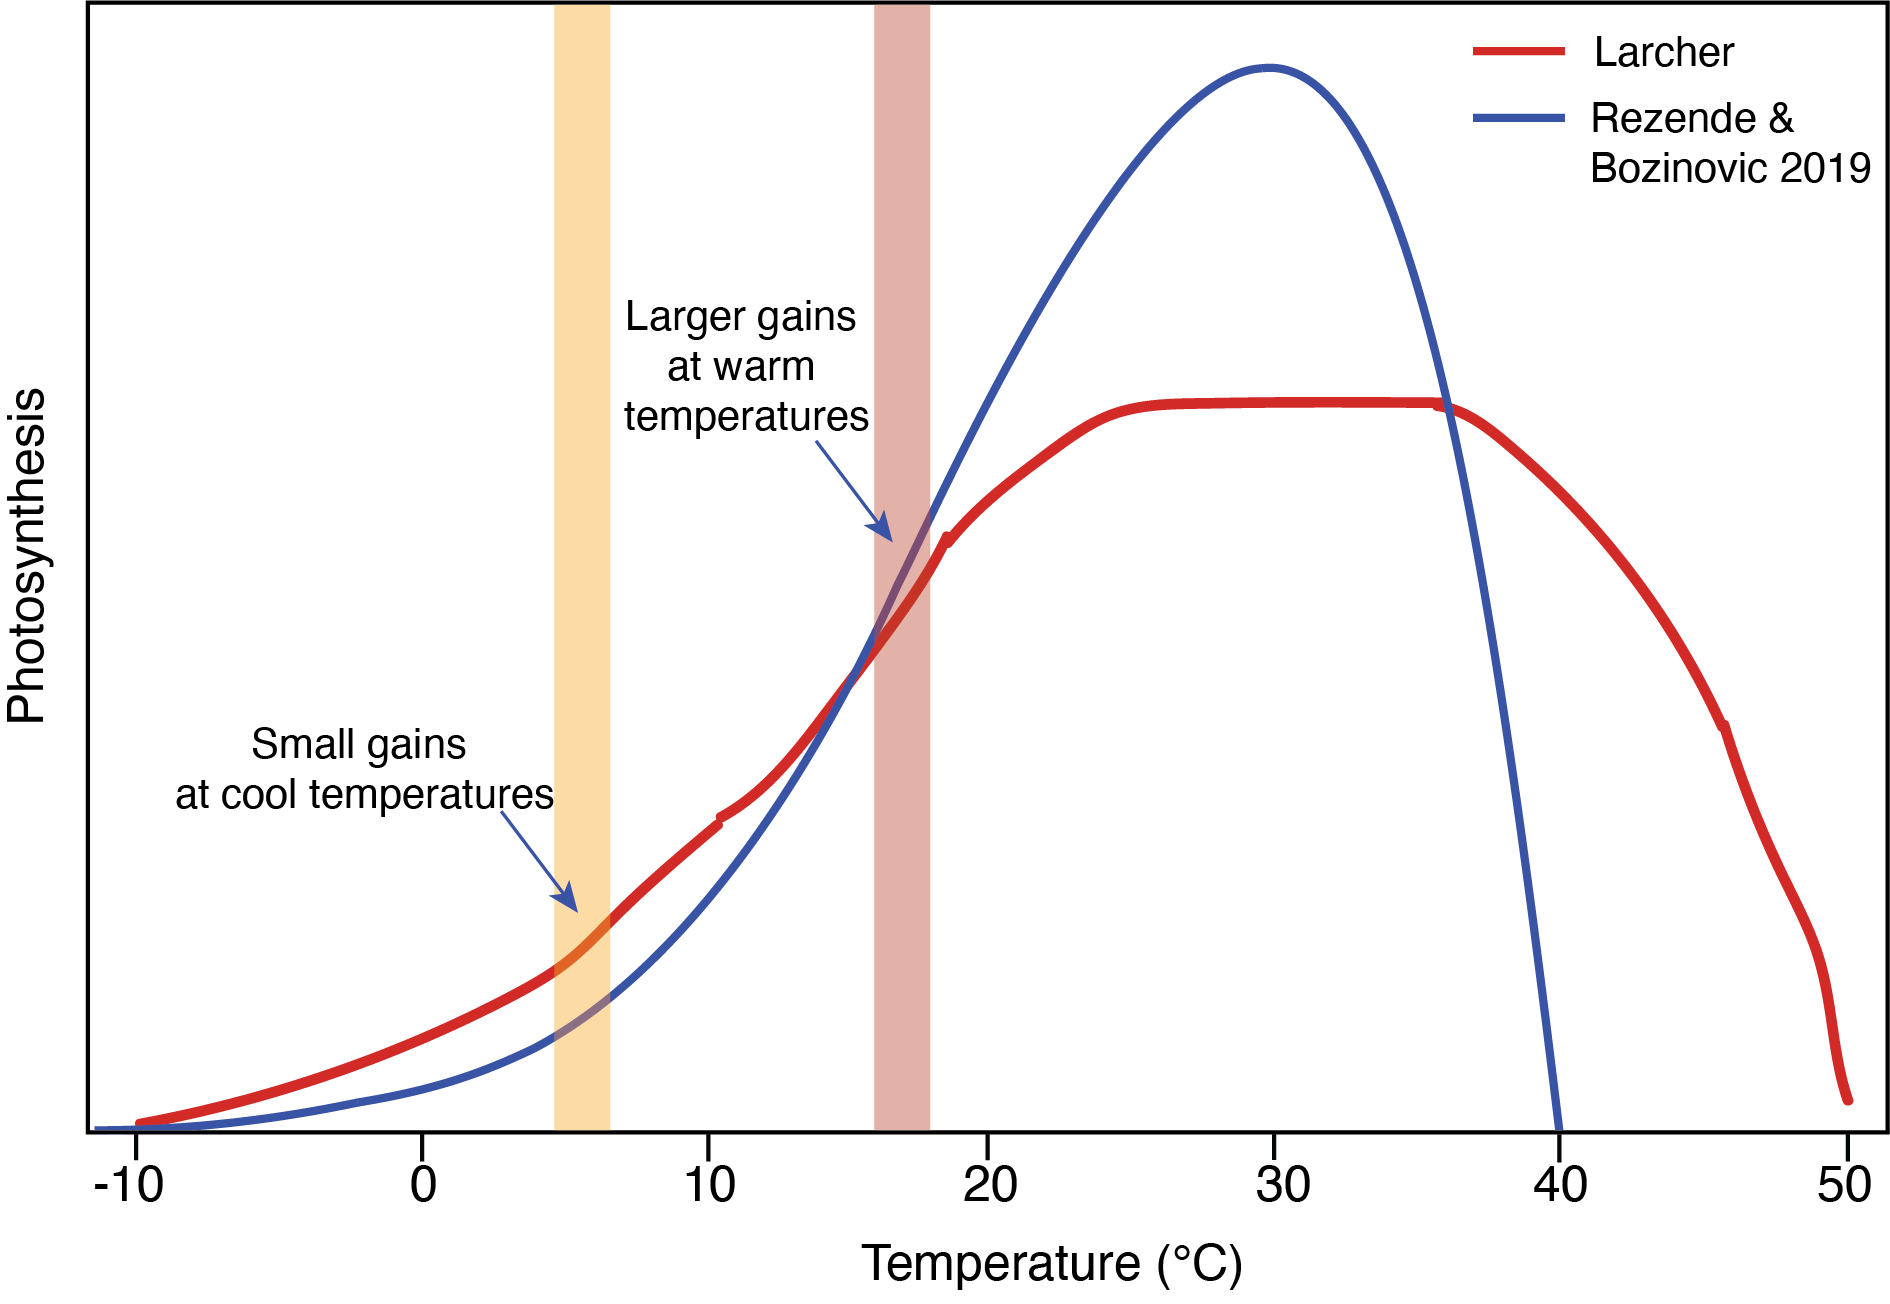
\includegraphics[width=0.75\textwidth]{..//figures/tempresponse/drafttempfig.png}
\caption{Growth responses to temperature depends on a suite of complex factors and is often represented as net photosynthesis, which has a non-linear response to temperature. This non-linearity means that increases in lower temperatures---such as those in the spring when much of growing season extensions may happen--have a lower absolute increase in photosynthesis compared to increases in later-season warmer temperatures. Because there is no unified model of this relationships, we show two different versions of the relationship based on \citet{larcher2003,rezende2019thermal}.}
\label{fig:temperaturecomplex}
\end{figure}

\clearpage
\begin{figure}[h!]
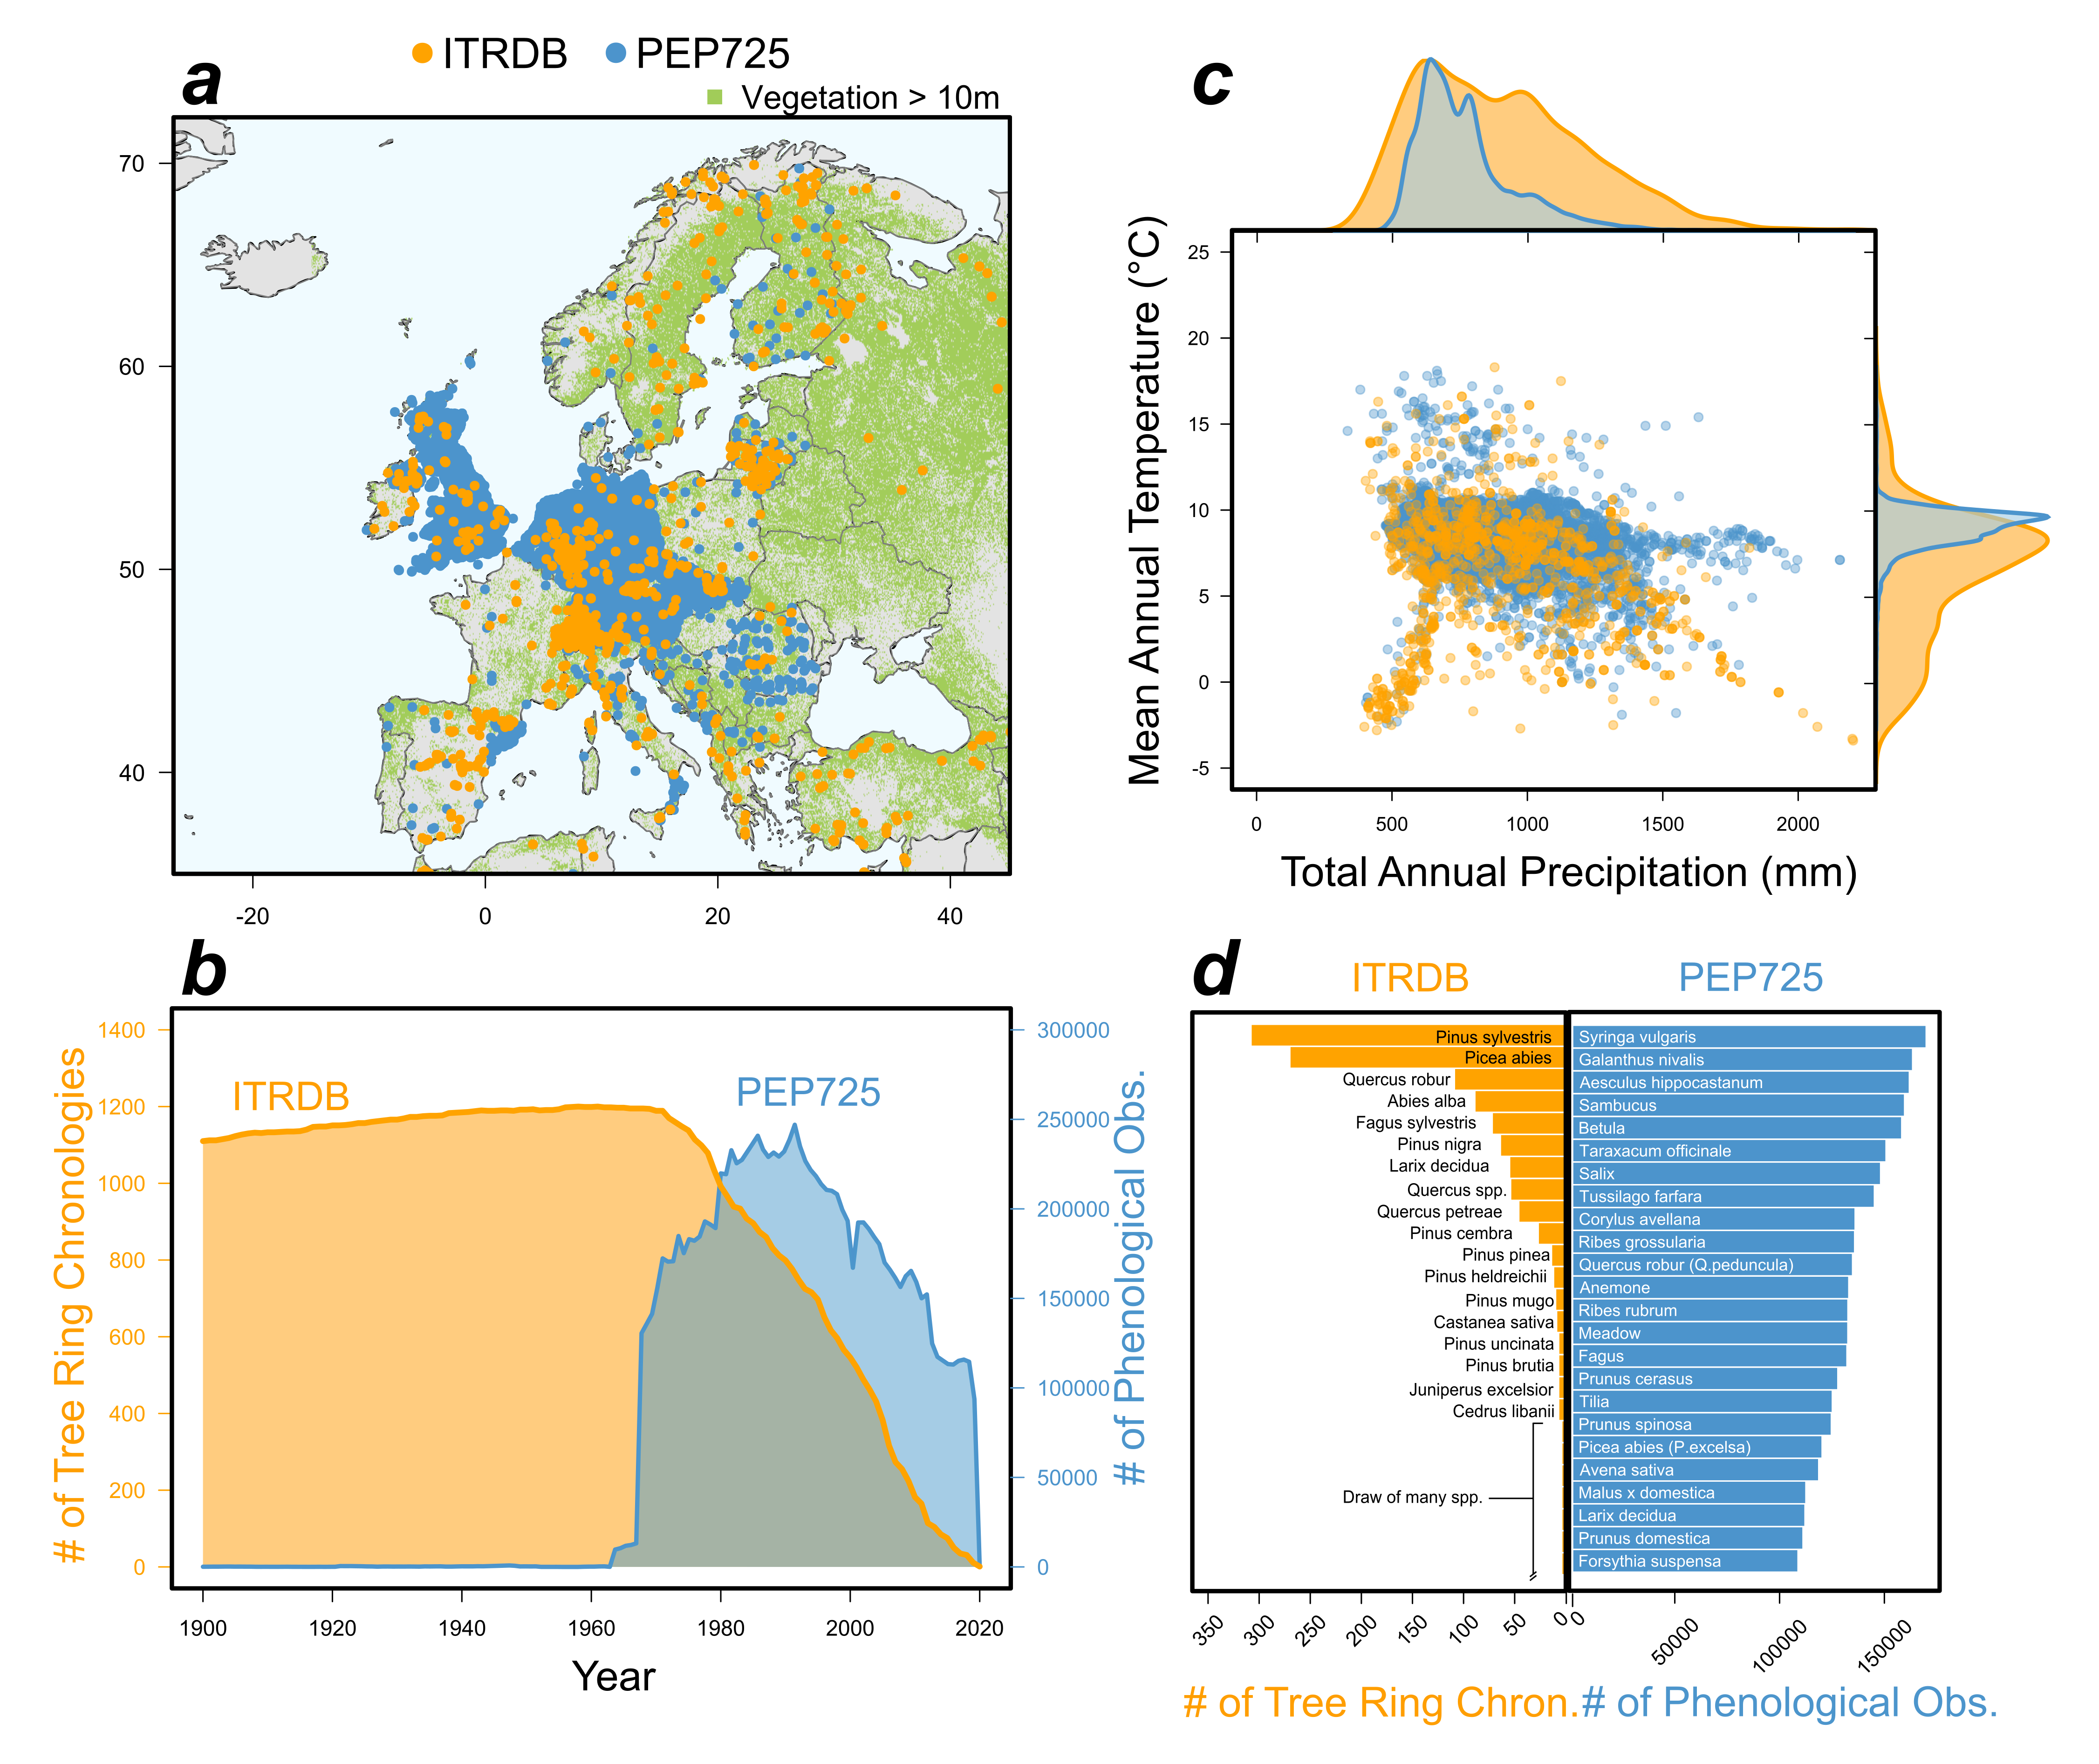
\includegraphics[width=1\textwidth]{..//figures/itrdbpep.png}
\caption{Data overlap between the two major databases of growth (International Tree Ring Data Bank, ITRDB, orange) and plant phenology (Pan European Phenology Project, PEP725, blue). Both databases are compared in terms of their spatial distributions (a), temporal overlaps (b), coverage of environmental conditions in climate space (c) and taxonomical representation (d). Note that the number of tree ring chronologies in (b) are composed by multiple trees per site, typically 10-20. Climatic data from Worldclim database ver. 2.1 at 2.5\degree grid resolution. PEP725 records in d) show the largest records for any given phenophase per species.}
\label{fig:itrbdpep}
\end{figure}

\iffalse
\begin{figure}[h!]
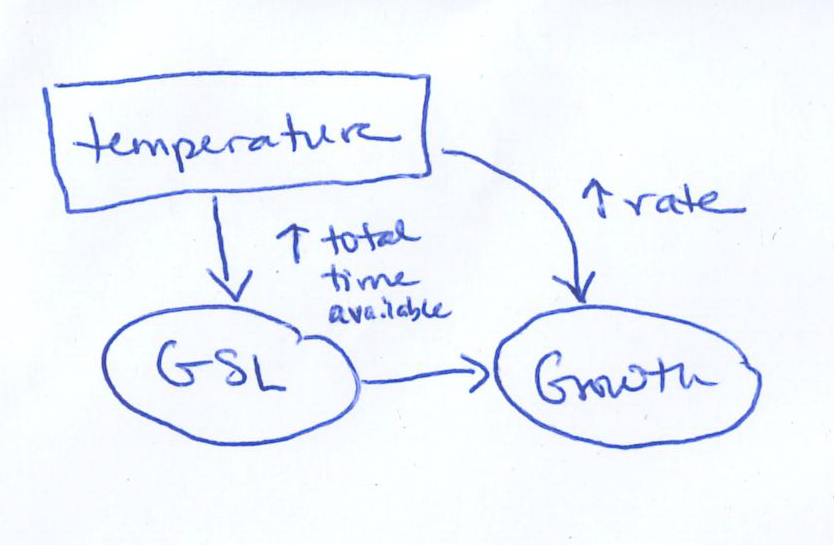
\includegraphics[width=0.5\textwidth]{..//figures/gsltogrowth/gsltogrowth_emw1a.png}
\caption{Idealized simplified version of the world, where resources (including water, N etc.) are abundant and temperatures are never too cool or too hot. In this world, temperature can increase growth directly (through increasing the speed of biological processes, up to some limit) and indirectly, but increasing the absolute available time for those processes to happen and lead to more growth.}
\label{fig:concepbiotime}
\end{figure}


\begin{figure}[h!]
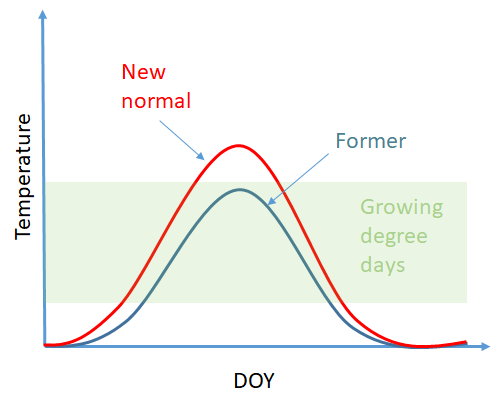
\includegraphics[width=0.75\textwidth]{..//figures/simpletempcurve_fromlucidboard.png}
\caption{Simplified version of how GDD works before and after climate change.}
\label{fig:simpletemp}
\end{figure}
\fi

\clearpage
\section{References}
\bibliography{..//bibtex/grephonbib}
\bibliographystyle{/Users/Lizzie/Documents/git/bibtex/styles/besjournals.bst} % pnas.bst says 87 refs on 18 May 2024





\end{document}


%%%%%%%%%%%%%%%%%%%%%%%%%%%%%%%
%% OLD text -- minus stuff I cut and used already (I think) %%
%%%%%%%%%%% %%%%%%%%%%%%%%%%%%%%

% Text that I cut from the previous draft but may want to REVIEW to see if it's worth fitting in somewhere

Internal/External drivers



 ...though how much longer seasons are depends on what events define the start and end (CITES). 

Perhaps most remarkably unmentioned in the current debate is the prevalence of species-level differences ....

Beyond genetic and developmental constraints, evolutionary history can constrain plant responses\todo{addcites}, though this is effectively unstudied currently as a controller of how growing season length may be limited in affecting growth. Yet most studies testing for such historical effects on plant responses find them... though this is effectively unstudied currently as a controller of how growing season length may be limited in affecting growth. Further, many physiological syntheses find results suggestive of strong phylogenetic relationships, but fail to discuss or test them \citep[e.g. discussions of evergreen versus deciduous phenology without testing for whether this is actually correlated with the deep in time split between gymnosperms and angiosperms,][]{way2010differential}. '

% Previous draft text ... 

\emph{How warmer temperatures increase tree growth, or not}


Elevation and latitude---two major factors that generally shorten seasons, and change a suite of climatic factors---generally lead to less annual growth (new Fig?). Most current work in dendrochronology assumes this relationship and focuses more on how climatic factors shift across these gradients\todo{addcites}. 



\emph{A cross-disciplinary framework for when longer seasons increase tree growth}


\emph{i. External drivers}

\emph{ii. Internal programming}



This focus on climatic signals in tree growth (measured by ring width) is the hallmark of dendrochronology, with the methods in the field generally designed around this aim. Statistical approaches attempt to remove periods of rapid growth with age. Sampling methods, at both the species and individual tree level, 
% Elevation and latitude---two major factors that generally shorten seasons, and change a suite of climatic factors---generally lead to less annual growth (new Fig?) though this relationship in reality may be more messy than many conceptual diagrams suggest. 


Additionally, observational studies must attempt to tease out effects of high temperatures that should accelerate the rate of plant growth, from longer seasons, and from temperatures that are too high and stall growth. Without a solid basis for the underlying temperature response curve, such attempts are likely non-identifiable statistically, and thus could easily report underlying correlations between predictors as signals of different temperature and season-length responses [\colorbox{orange}{More on VPD and/or xylogenesis here?}]. And these complexities must be addressed through a multi-species lens.

Only a handful of studies mentioned species differences, and rarely made predictions based on existing theory. Shifting investment in growth versus reproduction, differences in plant strategies and phylogeny all predict testable variation in how growing season length impacts growth, but have been almost wholly ignored in the current debate. We argue this is because of a lack of cross-disciplinary study. For example, while evolutionary history, ecology and life history theory all predict differences across species, the two major disciplines currently studying this---physiology and dendrochronology---generally study either one species\todo{addcites}, lump all species in a site\todo{addcites}, or divide by one trait \citep[e.g.][]{dow2022warm}. Research on trends over elevation, which seem foundational to understanding the growth x growing season length relationship, have been on a very limited species list---with almost no comparison across species. % Evolutionary history, ecology and life history theory all predict differences across species, but current analyses generally study either one species\todo{addcites}, or lump all species in a site\todo{addcites}.  

\emph{To the bat-mobile Robin! How to tackle this cross-disciplinary framework}


Dendrochronology provides an invaluable long-term perspective, but using it to understand tree growth beyond climatic factors will require new perspectives and approaches. As rings are easiest to observe in conifers, and conifers often exist in the most extreme climatic places (and thus have more clear signal of climate on growth), dendrochronology has limited data for species where phenology may be most strongly tied to growth---deciduous species, which are mostly angiosperms. Phenology and dendrochronology are somewhat unique fields in biology for their open data that is both geographically and temporally deep; yet the overlap in comparable data due to each field focusing mostly on different suites of species is incredibly limited (\colorbox{orange}{New fig here of PEP725 x ITRB data?}). Further, most standard statistical methods for `standardizing' tree ring data are focused on enhancing climatic signals---which could schmear insights into growing season length or other factors, especially for studies across populations \citep{de2022temperature}. The fundamental model of growth in dendrochronology could use revisiting, especially as new mechanistic understanding from physiology advances. Layering on the complexity of growth depending not only temperature and precipitation, but on vapor pressure deficit, as well as losses in growth that are more episodic (e.g. frost, disease) would help.

% 
ADD Both these [BIOTIC] drivers though can be more episodic and harder to measure, making them more difficult to easily test as mechanisms for limiting growth. In contrast, proxies for competition (such as surrounding tree density and identity), can be more easily measured, but are rarely studied. Mechanistic physiology studies rarely measure (or even include) competition and, given dendrochronology's focus on climatic signal through growth, the field similarly tries to avoid the study or impact of plant competition, even though it is foundational to forest dynamics. And ...  the very established method of merging into average site chronology reduces the chance of seeing competition or biotic factors in play.


Disentangling the effects of major drivers on growth---from growing season length, to temperature, moisture and constraints---likely requires experiments. To date, few experiments have teased out the effects of warmer temperatures versus an longer season, and none---to our knowledge---have carefully measured growth. Such experiments, however, will be critical in establishing a baseline understanding of the role of season length alone in determining growth. And they can compare species robustly. Advancing them to extend the season via early growth or delayed senescence, and layering on heat waves or drought treatments could provide comparable estimates and test lag effects (when sampled multiple years after the manipulations). While these are most easily done for juvenile trees, they could be done on adult trees (given the infrastructure investment), giving the opportunity to measure impacts on reproductive output as well. 
% Comparing the effects of various drivers on growth---from growing season length, to temperature, moisture and constraints---may be impossible from observational or experimental approaches alone. Each is limited ... 


